\chapter{Periodiciteit}\label{ch:b1:periodicity}

Lithium, natrium en kalium zijn zachte, glanzende metalen die aan de lucht
dof worden en met water reageren; fluor, chloor en broom zijn gekleurde,
bijtende niet-metalen die van bijna alles elektronen afpakken. Elk
drietal staat in één kolom van het periodiek systeem, en de leden van een
kolom lijken op elkaar, terwijl buren in een rij dat niet doen. Het
vorige hoofdstuk legde uit waarom: elementen van één kolom hebben dezelfde
configuratie van \omterm{def:b1:quantum-numbers:configuration}{valentie-elektronen}. Dit hoofdstuk zet die verklaring om
in getallen --- stralen, ionisatie-energieën, \omterm{def:b1:periodicity:electron-affinity}{elektronenaffiniteiten},
\omterm{def:b1:periodicity:electronegativity}{elektronegativiteiten} --- en in de trends waarmee een chemicus alleen uit
de plaats van een element kan voorspellen hoe groot zijn atomen zijn, hoe
gemakkelijk ze elektronen afstaan of opnemen, en naar welke kant de
elektronen van een binding overhellen.

\begin{recall}
Elke \omterm{def:b1:periodicity:table}{periode} begint met het vullen van een $n$\omterm{def:b1:quantum-numbers:orbital}{s-subschil} en eindigt met
een volle $n$\omterm{def:b1:quantum-numbers:orbital}{p-subschil}; het s-, p-, d- en \omterm{def:b1:periodicity:table}{f-blok} zijn 2, 6, 10 en 14
breed (\cref{prop:b1:quantum-numbers:table}). Boek 1 (jaar 11) beschreef
\omterm{def:b1:periodicity:electronegativity}{elektronegativiteit} als de neiging van een atoom om de elektronen van een
binding naar zich toe te trekken.
\end{recall}

\section{Het systeem, opgebouwd uit configuraties}

\begin{definition}[Periode, groep, blok]\label{def:b1:periodicity:table}
In het periodiek systeem staan de elementen in volgorde van toenemend
atoomnummer $Z$. Een \emph{periode}\index{periode} is een rij: de
elementen waarvan de valentieschil hetzelfde \omterm{def:b1:quantum-numbers:quantum-number}{hoofdkwantumgetal} $n$ heeft.
Een \emph{groep}\index{groep} is een kolom, genummerd van 1 tot 18: de
elementen met dezelfde valentieconfiguratie. Een \emph{blok}\index{blok}
is de verzameling elementen waarvan de laatst gevulde \omterm{def:b1:quantum-numbers:orbital}{subschil} van één
soort is, s, p, d of f.
\end{definition}

\begin{example}[Een plaats aflezen]\label{ex:b1:periodicity:position}
Seleen, $[\ce{Ar}]\,3\text{d}^{10} 4\text{s}^2 4\text{p}^4$, staat in
\omterm{def:b1:periodicity:table}{periode} 4 (valentieschil $n = 4$), in het \omterm{def:b1:periodicity:table}{p-blok} en in \omterm{def:b1:periodicity:table}{groep} 16 (twee
s-elektronen, tien d en vier p: $2 + 10 + 4$); zijn valentieconfiguratie
$n\text{s}^2 n\text{p}^4$ is die van zuurstof en zwavel erboven.
\end{example}

\begin{definition}[Metaal, niet-metaal, metalloïde]\label{def:b1:periodicity:metalloid}
Een metaal is een element waarvan de vaste stof elektriciteit geleidt en
waarvan de atomen gemakkelijk elektronen afstaan en kationen vormen; een
niet-metaal is een element dat niet geleidt (met uitzonderingen zoals
grafiet) en gemakkelijk elektronen opneemt of deelt. Een
\emph{metalloïde}\index{metalloide@metalloïde} is een element met een
tussenliggend karakter, een halfgeleider: boor, silicium, germanium,
arseen, antimoon en telluur.
\end{definition}

\begin{omfigure}
\omperiodictable[colour=metals, legend, f block=false]

{\small Metalen (de grote meerderheid), \omterm{def:b1:periodicity:metalloid}{metalloïden} langs een trap van
boor tot telluur, en niet-metalen rechtsboven. Het \omterm{def:b1:periodicity:table}{f-blok}, hier
weggelaten, bestaat uit metalen.}
\end{omfigure}

\section{Grootte: atoom- en ionstralen}

\begin{definition}[Afscherming, effectieve kernlading]\label{def:b1:periodicity:screening}
In een atoom met meerdere elektronen wordt een elektron aangetrokken door
de kern, met lading $Ze$, en afgestoten door de andere elektronen. De
binnenste elektronen heffen de aantrekking van de kern gedeeltelijk op:
dat is \emph{afscherming}\index{afscherming}. Het valentie-elektron
gedraagt zich alsof het een verminderde kernlading $Z^{*}e$ voelt, de
\emph{effectieve kernlading}\index{effectieve kernlading}, met
$Z^{*} < Z$. Elektronen van een binnenste schil schermen bijna volledig
af; elektronen van dezelfde schil maar een klein beetje.
\end{definition}

\begin{remark}[Een kwalitatief hulpmiddel]\label{rem:b1:periodicity:slater}
In dit boek wordt $Z^{*}$ kwalitatief gebruikt: langs een \omterm{def:b1:periodicity:table}{periode} neemt
$Z$ bij elke stap met één toe, terwijl het toegevoegde elektron, in
dezelfde schil, maar weinig afschermt, zodat de $Z^{*}$ die de
\omterm{def:b1:quantum-numbers:configuration}{valentie-elektronen} voelen toeneemt; in een groep naar beneden verandert
$Z^{*}$ weinig, maar de valentieschil $n$ wordt groter. Regels om
$Z^{*}$ uit de configuratie te berekenen (de regels van Slater) staan in
het deel van jaar 2.
\end{remark}

\begin{definition}[Covalente straal, ionstraal]\label{def:b1:periodicity:radius}
De \emph{covalente straal}\index{covalente straal} van een element is de
helft van de lengte van een enkelvoudige binding tussen twee van zijn
atomen: voor chloor de helft van de \ce{Cl-Cl}-afstand in \ce{Cl2}. De
\emph{ionstraal}\index{ionstraal} van een ion is het deel van de afstand
tussen naburige kationen en anionen in ionkristallen dat aan dat ion
wordt toegekend, volgens een afspraak die de straal van één
referentie-ion (\ce{O^{2-}}) vastlegt; hij hangt licht af van het aantal
buren.
\end{definition}

\begin{example}[De halogenen]\label{ex:b1:periodicity:halogen-radii}
De bindingslengten van \ce{F2}, \ce{Cl2}, \ce{Br2} en \ce{I2} zijn 141.2,
198.8, 228.1 en \qty{266.6}{pm}, zodat de covalente stralen 71, 99, 114
en \qty{133}{pm} zijn: elke stap omlaag in de groep voegt een schil en
ongeveer \qty{20}{pm} of meer toe.
% ledger: re:F2, re:Cl2, re:Br2, re:I2
\end{example}


\begin{proposition}[Trends in de straal]\label{prop:b1:periodicity:radius-trend}
Atoomstralen nemen langs een \omterm{def:b1:periodicity:table}{periode} van links naar rechts af en in een
groep van boven naar beneden toe. Een kation is kleiner dan zijn atoom,
een anion groter; in een iso-elektronische reeks (ionen met dezelfde
configuratie) neemt de straal af naarmate $Z$ toeneemt.
\end{proposition}

\begin{proof}[Redenering]
De grootte van een atoom is de grootte van zijn valentieorbitalen, die
krimpen als $Z^{*}$ groeit en zwellen als $n$ groeit. Langs een \omterm{def:b1:periodicity:table}{periode}
ligt $n$ vast en groeit $Z^{*}$: de atomen trekken samen. In een groep
naar beneden groeit $n$ bij elke stap met één, wat zwaarder weegt dan de
kleine verandering van $Z^{*}$. Een kation heeft zijn valentieschil
verloren, of elektronen die elkaar afstootten; een anion heeft een
elektron gewonnen dat de andere afstoot. In een iso-elektronische reeks
worden dezelfde elektronen vastgehouden door een kern met groeiende
lading.
\end{proof}

\begin{omfigure}
\begin{tikzpicture}[font=\small, x=1pt, y=1pt]
  % ledger: rion:O2-VI, rion:F-VI, rion:Na+VI, rion:Mg2+VI, rion:Al3+VI
  % radii in pm drawn at 0.30 pt per pm (circles to scale)
  \foreach \x/\r/\lab/\v in {40/140/\ce{O^{2-}}/140, 130/133/\ce{F-}/133,
      210/102/\ce{Na+}/102, 275/72/\ce{Mg^{2+}}/72, 325/53.5/\ce{Al^{3+}}/54} {
    \draw[fill=omDef!20, draw=omDef!70!black] (\x,0) circle ({0.30*\r});
    \node at (\x,0) {\lab};
    \node[below] at (\x,-50) {\v\,pm};
  }
  \node[anchor=west, align=left] at (350,0) {elk tien elektronen,\\$Z = 8 \to 13$};
\end{tikzpicture}

{\small De iso-elektronische reeks $1\text{s}^2 2\text{s}^2 2\text{p}^6$,
op schaal getekend (ionstralen voor zes buren). Dezelfde tien elektronen
krimpen naarmate de kernlading groeit.}
\end{omfigure}

\section{Energieën: ionisatie en elektronenaffiniteit}

\begin{definition}[Ionisatie-energieën]\label{def:b1:periodicity:ionisation-energy}
De \emph{eerste ionisatie-energie}\index{eerste ionisatie-energie} $E_{i1}$
van een element is de energie die nodig is om één elektron te verwijderen
uit het geïsoleerde atoom in zijn \omterm{def:b1:quantum-numbers:energy-level}{grondtoestand}, in de gasfase:
\[
  \ce{X(g) -> X+(g) + e-}, \qquad E_{i1} = E(\ce{X+}) + E(\ce{e-}) - E(\ce{X}) > 0 .
\]
De \emph{opeenvolgende ionisatie-energieën}\index{opeenvolgende ionisatie-energieen@opeenvolgende ionisatie-energieën}
$E_{i2}, E_{i3}, \dots$ verwijderen het tweede, het derde
elektron\dots\ uit \ce{X+}, \ce{X^{2+}}\dots\ Ze worden opgegeven in
elektronvolt per atoom of in kilojoule per mol
($\qty{1}{eV} \leftrightarrow \qty{96.49}{kJ/mol}$).
% ledger: const:NA, const:e (1 eV x N_A = 96.485 kJ/mol)
\end{definition}

\begin{omfigure}
\begin{tikzpicture}
\begin{axis}[
  width=0.92\linewidth, height=6.4cm,
  xmin=0, xmax=37, ymin=0, ymax=27,
  axis x line=bottom, axis y line=left,
  xlabel={atoomnummer $Z$}, ylabel={$E_{i1}$ (eV)},
  xtick={2,10,18,36}, ytick={0,5,10,15,20,25},
  tick label style={font=\small}, label style={font=\small},
  clip=false]
\addplot[omDef, thick, mark=*, mark size=1.3pt] table[x=Z, y=IE_eV] {figdata/out/bachelor-1-ionisation-energies.dat};
\node[font=\small, anchor=south] at (axis cs:2,24.6) {He};
\node[font=\small, anchor=south] at (axis cs:10,21.6) {Ne};
\node[font=\small, anchor=south] at (axis cs:18,15.8) {Ar};
\node[font=\small, anchor=south] at (axis cs:36,14.0) {Kr};
\node[font=\small, anchor=north] at (axis cs:3,5.2) {Li};
\node[font=\small, anchor=north] at (axis cs:11,4.9) {Na};
\node[font=\small, anchor=north] at (axis cs:19,4.1) {K};
\node[font=\small, anchor=north] at (axis cs:31,5.8) {Ga};
\node[font=\small, anchor=north] at (axis cs:5,7.9) {B};
\node[font=\small, anchor=north] at (axis cs:8,13.2) {O};
\node[font=\small, anchor=north west] at (axis cs:13.1,6.0) {Al};
\node[font=\small, anchor=north] at (axis cs:16,9.9) {S};
\node[font=\small, anchor=south] at (axis cs:26,8.0) {3d-metalen};
\end{axis}
\end{tikzpicture}

{\small Eerste ionisatie-energieën van de eerste 36 elementen. Maxima bij
de edelgassen, minima bij de alkalimetalen; de kleine dalen bij B, Al, Ga
en bij O, S zijn de subschileffecten van
\cref{prop:b1:periodicity:ie-anomalies}.}
\end{omfigure}

\begin{proposition}[Trends in de ionisatie-energie]\label{prop:b1:periodicity:ie-trend}
De \omterm{def:b1:periodicity:ionisation-energy}{eerste ionisatie-energie} neemt langs een \omterm{def:b1:periodicity:table}{periode} toe, van het
alkalimetaal tot het edelgas, en neemt in een groep naar beneden af. De
\omterm{def:b1:periodicity:ionisation-energy}{opeenvolgende ionisatie-energieën} nemen altijd toe,
$E_{i1} < E_{i2} < \dots$, en maken een sprong met een grote factor
wanneer het verwijderde elektron tot een binnenste schil behoort.
\end{proposition}

\begin{proof}[Redenering]
Een elektron verwijderen is gemakkelijker als het ver van de kern zit en
een kleine $Z^{*}$ voelt: langs een \omterm{def:b1:periodicity:table}{periode} groeit $Z^{*}$ en krimpt de
straal; in een groep naar beneden groeit de straal. Elk volgend elektron
wordt weggetrokken uit een ion met een hogere lading en een kleinere
omvang, en kost dus meer; zodra de valentieschil leeg is, komt het
volgende elektron uit een schil met kleinere $n$, veel dichter bij de
kern en nauwelijks afgeschermd.
\end{proof}

\begin{example}[Magnesium]\label{ex:b1:periodicity:magnesium}
De \omterm{def:b1:periodicity:ionisation-energy}{opeenvolgende ionisatie-energieën} van magnesium zijn 7.65, 15.04,
80.14 en \qty{109.27}{eV}. De verhouding $E_{i2}/E_{i1} \approx 2$ is
gematigd; $E_{i3}/E_{i2} \approx 5.3$ is een sprong: het derde elektron
komt uit de 2p-romp. Magnesium staat zijn twee 3s-elektronen af en stopt
bij \ce{Mg^{2+}}, met de edelgasconfiguratie van neon.
% ledger: ie:Mg, ie2:Mg, ie3:Mg, ie4:Mg
\end{example}

\begin{omfigure}
\begin{tikzpicture}
\begin{axis}[
  width=0.55\linewidth, height=5.2cm, ybar, bar width=14pt,
  xmin=0.4, xmax=4.6, ymin=1, ymax=300, ymode=log,
  axis x line=bottom, axis y line=left,
  xlabel={verwijderd elektron}, ylabel={$E_{i}$ (eV)},
  xtick={1,2,3,4}, xticklabels={1e,2e,3e,4e},
  tick label style={font=\small}, label style={font=\small},
  nodes near coords={\pgfmathprintnumber[fixed, fixed zerofill, precision=2]{\pgfplotspointmeta}},
  nodes near coords style={font=\scriptsize},
  point meta=rawy]
\addplot[fill=omDef!40, draw=omDef] table[x=k, y=IE_eV] {figdata/out/bachelor-1-ionisation-energies-mg.dat};
\end{axis}
\end{tikzpicture}

{\small \omterm{def:b1:periodicity:ionisation-energy}{Opeenvolgende ionisatie-energieën} van magnesium (logaritmische
as). De derde is vijf keer de tweede: de 3s-schil is leeg en de romp is
bereikt.}
\end{omfigure}

\begin{proposition}[Twee dalen langs een periode]\label{prop:b1:periodicity:ie-anomalies}
Langs de \omterm{def:b1:periodicity:table}{perioden} 2 en 3 daalt de \omterm{def:b1:periodicity:ionisation-energy}{eerste ionisatie-energie} licht van
\omterm{def:b1:periodicity:table}{groep} 2 naar \omterm{def:b1:periodicity:table}{groep} 13 (\ce{Be} naar \ce{B}, \ce{Mg} naar \ce{Al}) en van
\omterm{def:b1:periodicity:table}{groep} 15 naar \omterm{def:b1:periodicity:table}{groep} 16 (\ce{N} naar \ce{O}, \ce{P} naar \ce{S}).
\end{proposition}

\begin{proof}[Redenering]
In \ce{B} en \ce{Al} is het verwijderde elektron het eerste p-elektron,
hoger in energie dan de s-elektronen van \ce{Be} en \ce{Mg}. In \ce{O}
en \ce{S} is het verwijderde elektron het vierde p-elektron, het eerste
dat een orbitaal deelt (\omorbs{ud,u,u}): door de afstoting met zijn
partner is het gemakkelijker te verwijderen dan een elektron van de half
gevulde \omterm{def:b1:quantum-numbers:orbital}{subschil} van \ce{N} of \ce{P} (\omorbs{u,u,u}).
% ledger: ie:Be, ie:B, ie:N, ie:O, ie:Mg, ie:Al, ie:P, ie:S
\end{proof}


\begin{definition}[Elektronenaffiniteit]\label{def:b1:periodicity:electron-affinity}
De \emph{elektronenaffiniteit}\index{elektronenaffiniteit} $E_{ea}$ van
een element is de energie die vrijkomt wanneer een geïsoleerd atoom in
zijn \omterm{def:b1:quantum-numbers:energy-level}{grondtoestand} in de gasfase een elektron opneemt,
\[
  \ce{X(g) + e- -> X-(g)}, \qquad E_{ea} = E(\ce{X}) + E(\ce{e-}) - E(\ce{X-}) .
\]
Ze is positief wanneer het anion stabieler is dan het atoom met het
vrije elektron.
\end{definition}

\begin{example}[De halogenen en hun buren]\label{ex:b1:periodicity:ea}
De \omterm{def:b1:periodicity:electron-affinity}{elektronenaffiniteiten} van \ce{F}, \ce{Cl}, \ce{Br} en \ce{I} zijn
3.40, 3.61, 3.36 en \qty{3.06}{eV}, de grootste van alle elementen; die
van \ce{O} en \ce{S} zijn 1.44 en \qty{2.02}{eV}, die van \ce{C}
\qty{1.26}{eV}, die van \ce{Na} \qty{0.55}{eV}. Atomen die door een
elektron op te nemen een \omterm{def:b1:quantum-numbers:orbital}{subschil} voltooien (de halogenen), maken veel
energie vrij. Stikstof, beryllium, magnesium en de edelgassen vormen geen
stabiel anion in de gasfase: het extra elektron zou moeten paren in een
half gevulde \omterm{def:b1:quantum-numbers:orbital}{p-subschil} of in een nieuwe \omterm{def:b1:quantum-numbers:orbital}{subschil} terechtkomen. De
affiniteit van fluor is kleiner dan die van chloor, omdat het toegevoegde
elektron in de kleine 2p-schil wordt samengeperst.
% ledger: ea:F, ea:Cl, ea:Br, ea:I, ea:O, ea:S, ea:C, ea:Na
\end{example}


\section{Elektronegativiteit en polariseerbaarheid}

\begin{definition}[Elektronegativiteit]\label{def:b1:periodicity:electronegativity}
De \emph{elektronegativiteit}\index{elektronegativiteit} $\chi$ van een
element meet de neiging van zijn atomen om in een molecuul de elektronen
van de bindingen die ze vormen naar zich toe te trekken. Er zijn twee
schalen in gebruik.
\begin{itemize}
  \item Op de \emph{schaal van Pauling}\index{schaal van Pauling} worden
        verschillen gedefinieerd uit bindingsenergieën $D$:
        \[
          |\chi_A - \chi_B| = \sqrt{\frac{\Delta E}{\qty{1}{eV}}}, \qquad
          \Delta E = D(\text{A--B}) - \tfrac12\big[D(\text{A--A}) +
          D(\text{B--B})\big],
        \]
        en de schaal is verankerd met $\chi(\ce{F}) = 3.98$.
  \item Op de \emph{schaal van Mulliken}\index{schaal van Mulliken} is
        $\chi_M = \tfrac12\,(E_{i1} + E_{ea})$, in elektronvolt.
\end{itemize}
\end{definition}

\begin{remark}[Waarom de extra bindingsenergie]\label{rem:b1:periodicity:pauling}
Als de twee atomen van een binding A--B haar elektronen even sterk
aantrokken, zou de bindingsenergie ongeveer het gemiddelde zijn van die
van A--A en B--B. Wanneer één atoom elektronegatiever is, krijgt de
binding een gedeeltelijk ionair karakter, $\ce{A^{\delta+}-B^{\delta-}}$,
waarvan de elektrostatische aantrekking energie toevoegt: $\Delta E > 0$
meet het ongelijke delen. De definitie van Mulliken zegt hetzelfde vanuit
de atomen: een atoom dat zijn eigen elektronen stevig vasthoudt ($E_i$
groot) en een extra elektron graag opneemt ($E_{ea}$ groot), trekt de
elektronen van een binding aan.
\end{remark}

\begin{omfigure}
% ledger: en:H, en:Li, en:Be, en:B, en:C, en:N, en:O, en:F, en:Na, en:Mg,
% en:Al, en:Si, en:P, en:S, en:Cl, en:K, en:Ca, en:Ga, en:Ge, en:As, en:Se,
% en:Br, en:Rb, en:Sr, en:In, en:Sn, en:Sb, en:Te, en:I, en:Cs, en:Ba
\omperiodictable[upto=56, f block=false, numbers=false, highlight colour=omDef!12,
  highlight={F,O,N,Cl}, values={H/2.20,Li/0.98,Be/1.57,B/2.04,C/2.55,N/3.04,O/3.44,F/3.98,
  Na/0.93,Mg/1.31,Al/1.61,Si/1.90,P/2.19,S/2.58,Cl/3.16,K/0.82,Ca/1.00,Ga/1.81,Ge/2.01,
  As/2.18,Se/2.55,Br/2.96,Rb/0.82,Sr/0.95,In/1.78,Sn/1.96,Sb/2.05,Te/2.10,I/2.66,
  Cs/0.79,Ba/0.89}]

{\small \omterm{def:b1:periodicity:electronegativity}{Elektronegativiteiten} volgens Pauling van de hoofdgroepelementen
(het \omterm{def:b1:periodicity:table}{d-blok} is leeg gelaten). Ze nemen toe van links naar rechts en van
onder naar boven; de vier elektronegatiefste elementen, F, O, Cl en N,
zijn gearceerd.}
\end{omfigure}

\begin{proposition}[Trends in de elektronegativiteit]\label{prop:b1:periodicity:en-trend}
De \omterm{def:b1:periodicity:electronegativity}{elektronegativiteit} neemt langs een \omterm{def:b1:periodicity:table}{periode} toe en in een groep naar
beneden af: fluor is het elektronegatiefste element, cesium en francium
de minst elektronegatieve. Het verschil $\Delta\chi$ tussen twee
gebonden atomen bepaalt het karakter van de binding: $\Delta\chi < 0.4$
vrijwel apolair covalent, $0.4 < \Delta\chi < 1.7$ polair covalent,
$\Delta\chi > 1.7$ overwegend ionair --- drie gebieden van een continuüm,
geen scherp afgebakende klassen.
\end{proposition}

\begin{example}[Drie bindingen]\label{ex:b1:periodicity:bonds}
\ce{C-H}: $\Delta\chi = 2.55 - 2.20 = 0.35$, vrijwel apolair;
\ce{O-H}: $3.44 - 2.20 = 1.24$, polair, met een negatieve partiële
lading op het zuurstofatoom; \ce{Na-Cl}: $3.16 - 0.93 = 2.23$, ionair.
% ledger: en:C, en:H, en:O, en:Na, en:Cl
\end{example}


\begin{definition}[Polariseerbaarheid]\label{def:b1:periodicity:polarisability}
De \emph{polariseerbaarheid}\index{polariseerbaarheid} van een atoom, ion
of molecuul meet hoe gemakkelijk zijn elektronenwolk door een elektrisch
veld wordt vervormd --- het veld van een naburig ion of een naburige
dipool. Een polariseerbaar deeltje krijgt in een veld een geïnduceerd
dipoolmoment dat evenredig is met het veld.
\end{definition}

\begin{proposition}[Trends in de polariseerbaarheid]\label{prop:b1:periodicity:polarisability-trend}
De \omterm{def:b1:periodicity:polarisability}{polariseerbaarheid} groeit met de omvang van de elektronenwolk en met
het aantal elektronen, en neemt af met de lading van de kern die ze
vasthoudt: ze neemt in een groep naar beneden toe ($\ce{F-} < \ce{Cl-} < \ce{Br-} <
\ce{I-}$), anionen zijn veel polariseerbaarder dan kationen, en grote,
zachte anionen zoals \ce{I-} zijn de polariseerbaarste gangbare
deeltjes.
\end{proposition}

\begin{example}[Waarom polariseerbaarheid ertoe doet]\label{ex:b1:periodicity:pol}
De londonaantrekking tussen moleculen, het onderwerp van
\cref{ch:b1:intermolecular-forces-solvents}, groeit met de
\omterm{def:b1:periodicity:polarisability}{polariseerbaarheid}: dijood is bij kamertemperatuur een vaste stof,
dichloor een gas. In een ionkristal polariseert een klein, sterk geladen
kation een groot anion en geeft het de binding enig covalent karakter:
het falen van het eenvoudige ionaire model dat we in
\cref{ch:b1:crystals-ionic-covalent} tegenkomen.
\end{example}

\begin{history}[De schaal van Pauling, 1932]
In 1932 merkte de Amerikaanse chemicus Linus Pauling op dat de energie
van een binding tussen twee verschillende atomen bijna altijd groter is
dan het gemiddelde van de energieën van de twee symmetrische bindingen,
en bouwde hij uit dat overschot de eerste schaal van \omterm{def:b1:periodicity:electronegativity}{elektronegativiteit}.
Zijn schaal, herzien naarmate betere bindingsenergieën werden gemeten,
staat nog steeds in elke tabel. Pauling kreeg in 1954 de Nobelprijs voor
Scheikunde, voor zijn werk over de chemische binding, en in 1962 de
Nobelprijs voor de Vrede.
\end{history}

\begin{omfigure}
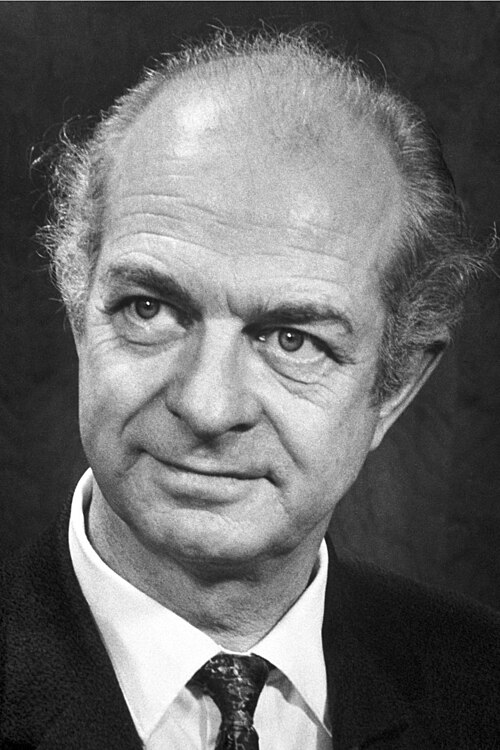
\includegraphics[width=0.24\linewidth]{images/book2/pauling.jpg}

{\small Linus Pauling (1901--1994).}
\end{omfigure}

\section{Trends in het chemische karakter}

\begin{proposition}[Reducerend en oxiderend karakter]\label{prop:b1:periodicity:redox-trend}
Elementen met een lage ionisatie-energie en een lage
\omterm{def:b1:periodicity:electronegativity}{elektronegativiteit}, links in het systeem en onderaan hun groep, staan
gemakkelijk elektronen af: het zijn reducerende metalen (de alkalimetalen
het sterkst). Elementen met een hoge \omterm{def:b1:periodicity:electronegativity}{elektronegativiteit} en
\omterm{def:b1:periodicity:electron-affinity}{elektronenaffiniteit}, rechtsboven, nemen gemakkelijk elektronen op: het
zijn oxiderende niet-metalen (fluor, zuurstof en chloor het sterkst). De
edelgassen, met een hoge ionisatie-energie en geen affiniteit voor een
extra elektron, doen geen van beide.
\end{proposition}

\begin{method}[Een trend voorspellen uit de plaats]\label{met:b1:periodicity:predict}
Zo vergelijk je twee elementen voor een eigenschap die afhangt van de
greep van de kern op de \omterm{def:b1:quantum-numbers:configuration}{valentie-elektronen} (straal, $E_i$, $E_{ea}$,
$\chi$):
\begin{enumerate}
  \item staan ze in dezelfde groep, dan heeft het onderste de grotere
        $n$: grotere straal, kleinere $E_i$ en $\chi$;
  \item staan ze in dezelfde \omterm{def:b1:periodicity:table}{periode}, dan heeft het meest rechtse de
        grotere $Z^{*}$: kleinere straal, grotere $E_i$ en $\chi$;
  \item vergelijk anders elk van beide met het element op het kruispunt
        van zijn rij en de kolom van het andere;
  \item controleer op subschileffecten (begin van een \omterm{def:b1:quantum-numbers:orbital}{p-subschil}, eerste
        gepaarde p-elektron) voordat je iets over ionisatie-energieën
        besluit.
\end{enumerate}
\end{method}

\begin{example}[Lithium in een batterij]\label{ex:b1:periodicity:lithium}
Lithium heeft de laagste \omterm{def:b1:periodicity:electronegativity}{elektronegativiteit} van \omterm{def:b1:periodicity:table}{periode} 2 en staat zijn
2s-elektron gemakkelijk af, terwijl het het lichtste metaal is: het
draagt per gram de meeste overdraagbare lading van alle elementen, en
daarom drijft het oplaadbare batterijen aan. Zijn \omterm{def:b1:periodicity:ionisation-energy}{eerste
ionisatie-energie}, \qty{5.39}{eV}, is groter dan die van natrium (5.14)
of kalium (4.34), en toch is het in water het sterkst reducerende
alkalimetaal, een paradox die wordt opgelost door de sterke hydratatie
van het kleine \ce{Li+}-ion (\cref{ch:b1:nernst}).
% ledger: ie:Li, ie:Na, ie:K
\end{example}


\section{Oefeningen}

\begin{exercise}[$\star$]\label{exo:b1:periodicity:1}
Geef de \omterm{def:b1:periodicity:table}{periode}, de groep en het \omterm{def:b1:periodicity:table}{blok} van calcium, ijzer, seleen en jood
($Z = 20, 26, 34, 53$), uitgaande van hun configuraties.
\end{exercise}

\begin{exercise}[$\star$]\label{exo:b1:periodicity:2}
Welk deeltje is in elk paar het grootste, en waarom? \ce{Na} of \ce{Cl};
\ce{Na} of \ce{Na+}; \ce{F-} of \ce{Cl-}; \ce{Na+} of \ce{Mg^{2+}}.
\end{exercise}

\begin{exercise}[$\star$]\label{exo:b1:periodicity:3}
De eerste ionisatie-energieën van \ce{Na}, \ce{Mg}, \ce{Al}, \ce{P},
\ce{S} en \ce{Ar} zijn 5.14, 7.65, 5.99, 10.49, 10.36 en
\qty{15.76}{eV}. Rangschik ze en wijs de twee afwijkingen van de
algemene trend aan.
\end{exercise}

\begin{exercise}[$\star$]\label{exo:b1:periodicity:4}
Definieer de \omterm{def:b1:periodicity:polarisability}{polariseerbaarheid} van een deeltje. Wat is polariseerbaarder,
\ce{F-} of \ce{I-}? \ce{Na+} of \ce{Cl-}? Verantwoord.
\end{exercise}

\begin{exercise}[$\star\star$]\label{exo:b1:periodicity:5}
De eerste vier ionisatie-energieën van een element uit \omterm{def:b1:periodicity:table}{periode} 3 zijn
5.99, 18.83, 28.45 en \qty{119.99}{eV}. Bereken de opeenvolgende
verhoudingen, en identificeer het element en het ion dat het vormt.
\end{exercise}

\begin{exercise}[$\star\star$]\label{exo:b1:periodicity:6}
Leg uit waarom chloor een grotere \omterm{def:b1:periodicity:electron-affinity}{elektronenaffiniteit} heeft dan fluor,
en waarom stikstof en magnesium geen stabiel anion in de gasfase vormen.
\end{exercise}

\begin{exercise}[$\star\star$]\label{exo:b1:periodicity:7}
Bereken de \omterm{def:b1:periodicity:electronegativity}{elektronegativiteiten} volgens Mulliken van natrium ($E_{i1} =
\qty{5.14}{eV}$, $E_{ea} = \qty{0.55}{eV}$) en chloor ($E_{i1} =
\qty{12.97}{eV}$, $E_{ea} = \qty{3.61}{eV}$). Wat zeggen ze over de
binding in \ce{NaCl}?
\end{exercise}

\begin{exercise}[$\star\star$]\label{exo:b1:periodicity:8}
Deel met de waarden volgens Pauling van \cref{ex:b1:periodicity:bonds} en $\chi(\ce{F})
= 3.98$ de bindingen \ce{H-F}, \ce{C-H}, \ce{Na-Cl}, \ce{C-Cl}
($\chi(\ce{Cl}) = 3.16$) en \ce{O-H} in, en geef het teken van de
partiële lading op elk atoom.
\end{exercise}

\begin{exercise}[$\star\star$]\label{exo:b1:periodicity:9}
De eerste ionisatie-energieën van \ce{Li}, \ce{Na} en \ce{K} zijn 5.39,
5.14 en \qty{4.34}{eV}. Verklaar de trend en voorspel of die van
rubidium boven of onder \qty{4.34}{eV} ligt.
\end{exercise}

\begin{exercise}[$\star\star\star$]\label{exo:b1:periodicity:10}
Zink ($Z = 30$) heeft een \omterm{def:b1:periodicity:ionisation-energy}{eerste ionisatie-energie} van \qty{9.39}{eV} en
gallium ($Z = 31$) van \qty{6.00}{eV}; arseen ($Z = 33$) \qty{9.79}{eV}
en seleen ($Z = 34$) \qty{9.75}{eV}. Verklaar beide dalingen met behulp
van de configuraties.
\end{exercise}

\begin{exercise}[$\star\star\star$]\label{exo:b1:periodicity:11}
Neem $D(\ce{H-H}) = \qty{436}{kJ/mol}$, $D(\ce{F-F}) =
\qty{158}{kJ/mol}$, $\chi(\ce{H}) = 2.20$ en $\chi(\ce{F}) = 3.98$, met
$\qty{1}{eV} = \qty{96.5}{kJ/mol}$. Schat met de definitie van Pauling
de bindingsenergie $D(\ce{H-F})$. Waarom is ze zoveel groter dan het
gemiddelde van de twee symmetrische bindingen?
\end{exercise}

\begin{exercise}[$\star\star\star$]\label{exo:b1:periodicity:12}
Voor krypton (3.00) en xenon (2.60) zijn \omterm{def:b1:periodicity:electronegativity}{elektronegativiteiten} volgens
Pauling getabelleerd, maar niet voor helium, neon of argon. Leg met de
definitie van de schaal uit waarom alleen een waarde gegeven kan worden
voor een element dat bindingen vormt, en waarom juist de zwaardere
edelgassen dat doen.
% ledger: en:Kr, en:Xe
\end{exercise}


\section{Probleem: het rekenwerk van Pauling}

\begin{problem}[{Weekendprobleem --- een onbekend element uit zijn
ionisatie-energieën, een reeks ionen met een even grote elektronenwolk,
twee schalen van elektronegativiteit, en het getal van Pauling voor de
H--Cl-binding}]
\label{pb:b1:periodicity:1}
Gegeven: $\qty{1}{eV}$ per deeltje komt overeen met \qty{96.485}{kJ/mol}.

\medskip
\noindent\textbf{Deel I --- Een onbekend element.}
De eerste vier ionisatie-energieën van een element X uit \omterm{def:b1:periodicity:table}{periode} 3 zijn
7.65, 15.04, 80.14 en \qty{109.27}{eV}.
\begin{enumerate}
  \item Waarom is elke ionisatie-energie groter dan de vorige?
  \item Bereken de verhoudingen $E_{i2}/E_{i1}$, $E_{i3}/E_{i2}$ en
        $E_{i4}/E_{i3}$.
  \item Leid de groep van X af en identificeer het element.
  \item Welk ion vormt X in zijn verbindingen? Geef de configuratie ervan.
  \item Is X een metaal of een niet-metaal? Verantwoord vanuit zijn plaats.
  \item Waarom kost het derde elektron zoveel meer dan het tweede?
\end{enumerate}

\medskip
\noindent\textbf{Deel II --- Tien elektronen.}
De ionstralen (zes buren) van \ce{O^{2-}}, \ce{F-}, \ce{Na+},
\ce{Mg^{2+}} en \ce{Al^{3+}} zijn 140, 133, 102, 72 en \qty{54}{pm}.
\begin{enumerate}[resume]
  \item Toon aan dat deze ionen dezelfde configuratie hebben.
  \item Verklaar de rangorde van de stralen.
  \item Welk van de vijf ionen is het polariseerbaarst, en waarom?
  \item Bereken de verhouding van de grootste tot de kleinste straal.
  \item De bindingslengte van \ce{Cl2} is \qty{198.8}{pm} en de straal van
        \ce{Cl-} \qty{181}{pm}. Bereken de \omterm{def:b1:periodicity:radius}{covalente straal} van chloor en
        vergelijk.
  \item Rangschik \ce{Cl-}, \ce{Na+} en \ce{Mg^{2+}} zonder verdere
        gegevens naar grootte.
\end{enumerate}

\medskip
\noindent\textbf{Deel III --- De \omterm{def:b1:periodicity:electronegativity}{schaal van Mulliken}.}
\begin{center}
\small
\begin{tabular}{lccccc}
\hline
element & \ce{F} & \ce{Cl} & \ce{Br} & \ce{O} & \ce{C} \\
\hline
$E_{i1}$ (eV) & 17.42 & 12.97 & 11.81 & 13.62 & 11.26 \\
$E_{ea}$ (eV) & 3.40 & 3.61 & 3.36 & 1.44 & 1.26 \\
$\chi$ (Pauling) & 3.98 & 3.16 & 2.96 & 3.44 & 2.55 \\
\hline
\end{tabular}
\end{center}
% ledger: ie:F, ie:Cl, ie:Br, ie:O, ie:C, ea:F, ea:Cl, ea:Br, ea:O, ea:C,
% en:F, en:Cl, en:Br, en:O, en:C
\begin{enumerate}[resume]
  \item Bereken de \omterm{def:b1:periodicity:electronegativity}{elektronegativiteiten} volgens Mulliken van de vijf
        elementen.
  \item Rangschik ze op elke schaal. Welk element staat op een andere
        plaats?
  \item Bereken de verhouding $\chi_{\text{Pauling}}/\chi_M$ voor de drie
        halogenen. Wat valt op?
  \item Geef een reden waarom zuurstof afwijkt van de regel van de
        halogenen (kijk naar zijn \omterm{def:b1:periodicity:electron-affinity}{elektronenaffiniteit}).
  \item Welk atoom draagt de negatieve partiële lading in \ce{HCl}? En in
        \ce{ClF}?
  \item Is, met de getabelleerde waarden ($\chi(\ce{H}) = 2.20$), de
        \ce{H-Cl}-binding apolair, polair covalent of ionair?
\end{enumerate}

\medskip
\noindent\textbf{Deel IV --- Het getal van Pauling voor H--Cl.}
De standaardvormingsenthalpieën van \ce{H(g)}, \ce{Cl(g)} en
\ce{HCl(g)} bij \qty{298}{K} zijn 218.0, 121.3 en \qty{-92.3}{kJ/mol};
die van \ce{H2(g)} en \ce{Cl2(g)} zijn nul. De bindingsenergie van een
molecuul wordt gelijkgesteld aan de enthalpie van zijn dissociatie in
atomen.
% ledger: janaf:H, janaf:Cl, janaf:HCl
\begin{enumerate}[resume]
  \item Bereken $D(\ce{H-H})$ uit \ce{H2(g) -> 2H(g)}.
  \item Bereken $D(\ce{Cl-Cl})$.
  \item Bereken $D(\ce{H-Cl})$ uit \ce{HCl(g) -> H(g) + Cl(g)}.
  \item Bereken de overschotenergie $\Delta E$ van Pauling in kJ/mol, en
        toon aan dat ze gelijk is aan $-\Delta_f H(\ce{HCl})$.
  \item Reken $\Delta E$ om naar elektronvolt.
  \item Bereken $|\chi(\ce{Cl}) - \chi(\ce{H})|$ en vergelijk met het
        verschil van de getabelleerde waarden, $3.16 - 2.20$.
\end{enumerate}
\end{problem}
